\documentclass[12pt,fleqn]{article}\usepackage{../../common}
\begin{document}

$$ {\displaystyle {\ddot {\vec {r_{1}}}}={\frac {Gm_{2}}{|{\vec
        {r_{1}}}-{\vec {r_{2}}}|^{3}}}({\hat {r_{2}}}-{\hat {r_{1}}})}
$$

$${\displaystyle {\ddot {\vec {r_{2}}}}={\frac {Gm_{2}}{|{\vec
        {r_{1}}}-{\vec {r_{2}}}|^{3}}}({\hat {r_{1}}}-{\hat {r_{2}}})}
$$ 



\begin{minted}[fontsize=\footnotesize]{python}
from scipy.integrate import odeint
import matplotlib.pyplot as plt
import numpy as np

m1 = 1
m2 = 1

def twobody(state, t):
    x1 = np.array([state[0], state[1], state[2]])
    v1 = np.array([state[3], state[4], state[5]])
    x2 = np.array([state[6], state[7], state[8]])
    v2 = np.array([state[9], state[10], state[11]])

    r = x2-x1
    r = np.sqrt(np.sum(r*r))

    x1d = v1
    v1d = m2*(x2-x1)/(r*r*r)
    x2d = v2
    v2d = m1*(x1-x2)/(r*r*r)

    return [x1d[0],x1d[1],x1d[2],v1d[0],v1d[1],v1d[2],x2d[0],x2d[1],x2d[2],v2d[0],v2d[1],v2d[2]]

state0 = [0.0, 0.0, 0.0, 0.0,0.0,0.0, 1,0,0, 0.0,1.0,0.0]

t = np.arange(0.0,100.0, 0.01)
state = odeint(twobody, state0, t)

from mpl_toolkits.mplot3d import Axes3D
fig = plt.figure()
ax = fig.gca(projection='3d')
ax.plot(state[:,6]-state[:,0], state[:,7]-state[:,1], state[:,8]-state[:,2])
ax.set_xlabel('x')
ax.set_ylabel('y')
ax.set_zlabel('z')
plt.savefig('test_01.png')
\end{minted}

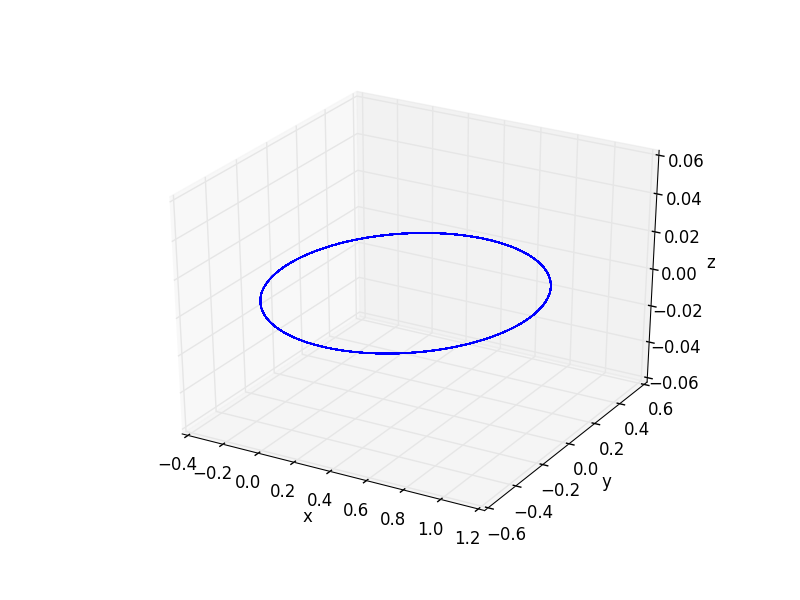
\includegraphics[height=6cm]{twobody_01.png}























\end{document}
